\section{Research Design}\label{research-design}

The study follows a design science research logic. The practical problem
is to enrich resource behaviour in process simulation while preserving
reproducibility and measurability. The resulting artifact is a
resource-centric multi-agent simulator with log-derived constraints and
an LLM-style local decision interface. Generated logs are evaluated
against held-out real logs using prototype metrics and formal BPS
quality measures.

Figure~\ref{fig:architecture} summarizes the central design choice: the
simulator places the LLM-style module inside a log-derived pipeline as a
constrained local decision component.

\begin{figure}[htbp]
\centering
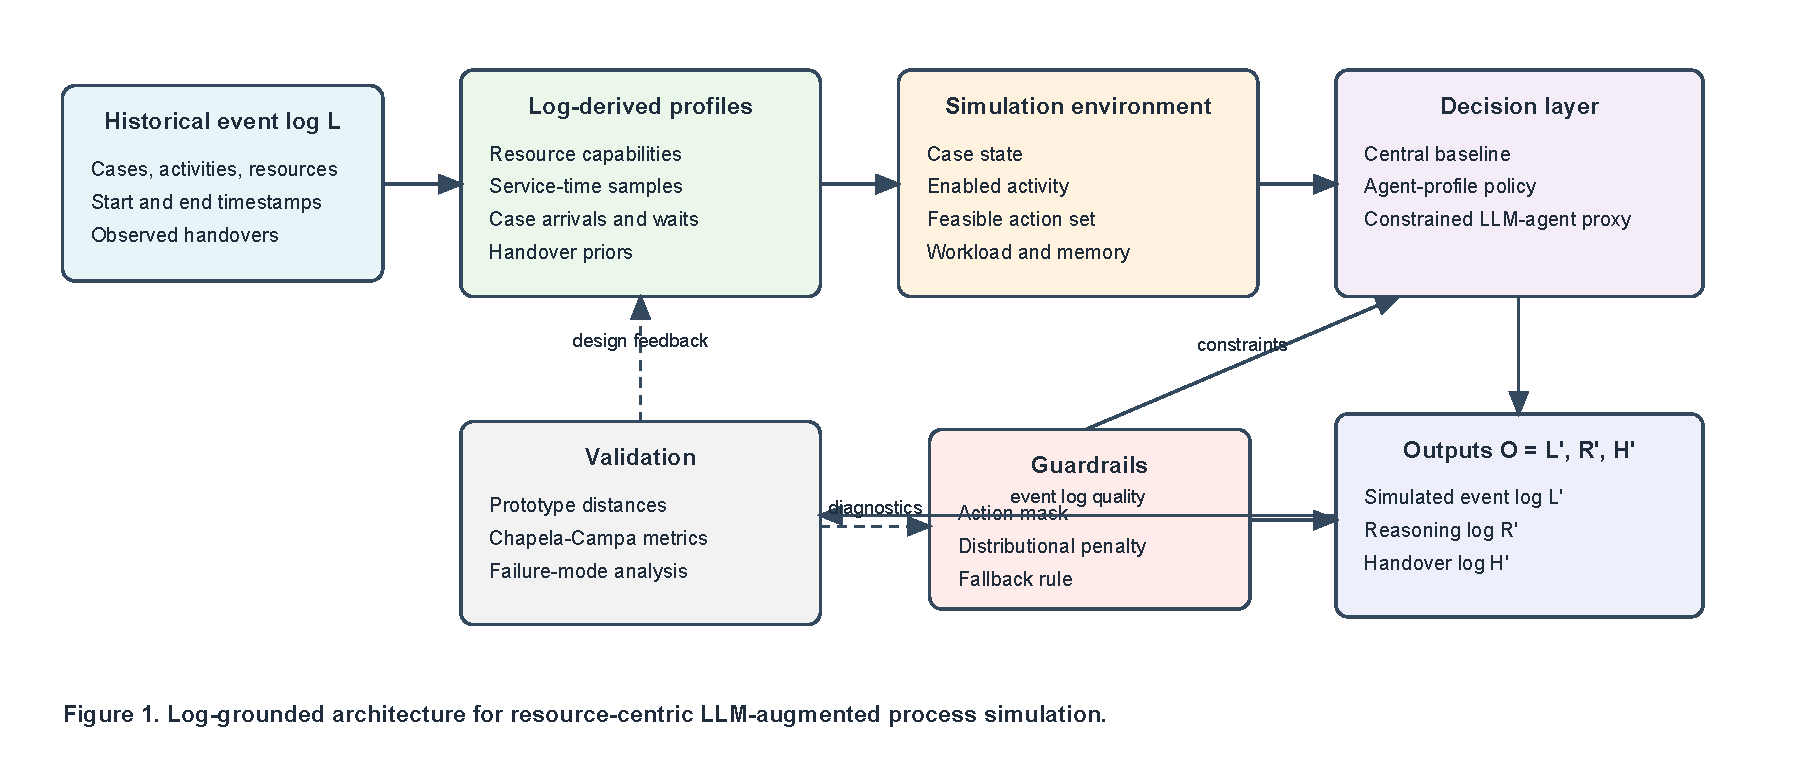
\includegraphics[width=\textwidth]{figures/figure1_architecture.pdf}
\caption{Architecture of the resource-centric LLM-augmented multi-agent process simulator. A historical event log is transformed into resource capabilities, timing samples, arrival and waiting-time samples, and activity-resource/handover priors. During simulation, the central baseline, agent-profile policy, LLM-agent proxy, and optional real-LLM condition choose among feasible local actions under shared event-log constraints. Guardrails include action masks, JSON validation for API-backed LLM calls, distributional penalties, and fallback rules. The simulator produces a process-mining-compatible event log and, for LLM-agent conditions, reasoning and handover logs. Generated outputs are evaluated through a dual framework covering BPS log quality, LLM-agent behavioural quality, and what-if response.}
\label{fig:architecture}
\end{figure}

The artifact is summarized as:

\[
H_{R-LLM} = (L, A, P_{env}, X, \Pi_{log}, M, B_{LLM}, S, O, V)
\]

where \(L\) is the input event log, \(A\) is the set of resource agents,
\(P_{env}\) describes the simulation environment including arrivals and
enabled activities, \(X\) is the case and event state, \(\Pi_{log}\)
contains log-derived priors, \(M\) is agent memory, \(B_{LLM}\) is the
LLM-style behaviour module, \(S\) is the simulator state transition
function, \(O\) is the output, and \(V\) is the validation framework.

Each agent \(a_i\) is represented by a profile:

\[
a_i = (s_i, c_i, \rho_i, m_i, b_i^{LLM})
\]

where \(s_i\) is the agent state, \(c_i\) contains capabilities and
processing-time samples, \(\rho_i\) contains local resource and handover
priors, \(m_i\) is memory, and \(b_i^{LLM}\) is the decision module.
In the current implementation, \(b_i^{LLM}\) is represented by the
deterministic LLM-agent proxy. The proxy receives a local state and
chooses only among feasible resources and activities. It cannot invent
activities, resources, or timestamps outside the learned simulation
structure.

The central design principle is:

\textbf{LLM agents should reason over log-grounded local feasible
actions, not freely generate process behaviour.}

The simulator produces three output types:

\[
O = (L', R', H')
\]

where \(L'\) is the simulated event log, \(R'\) is the reasoning log, and
\(H'\) is the handover log. \(L'\) supports process-mining and BPS
evaluation, whereas \(R'\) and \(H'\) expose local reasoning and
cross-resource transitions for LLM-agent conditions.
